\chapter{Систення інформація за допомогою бінарних дерев}
\nopagebreak[4]
\section*{Мета роботи}

\nopagebreak[4]
\section{Вступ}
\nopagebreak[4]
Дерево~--- це структура даних, що представляє собою сукупність елементів і відносин, що утворюють ієрархічну структуру цих елементів (рис.~\ref{f:tree1}). Кожен елемент дерева називається вершиною (вузлом) дерева. Вершини дерева з'єднані спрямованими дугами, які називають гілками дерева. Початковий вузол дерева називають коренем дерева, йому відповідає нульовий рівень. Листям дерева називають вершини, в які входить одна гілка і не виходить жодної гілки.

Кожне дерево має такі властивості:
\begin{itemize}
\item існує вузол, в який не входить ні однієї дуги (корінь);
    в кожну вершину, крім кореня, входить одна дуга.
\end{itemize}


Дерева особливо часто використовують на практиці при зображенні різних ієрархій.

\begin{figure}
\caption{Дерево}\label{f:tree1}
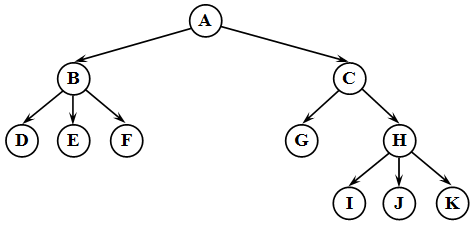
\includegraphics[width=13cm]{pic/31_01.png}

\end{figure}

\section{Ключові терміни}
\nopagebreak[4]




\section{Розширені теоретичні відомості}
\nopagebreak[4]




\section{Приклади обчислень}
\nopagebreak[4]




\subsection*{Контрольні запитання}
\nopagebreak[4]
\begin{enumerate}
\item ?
\end{enumerate}



